\section{Experiment}
\subsection{Experimental Settings} \label{exp_settings_large}
We conducted the experiments on the Google Web Treebank \cite{PM12}, consisting of the WSJ portion of the OntoNotes corpus and five additional web domains, with 48 dependency types. The models were trained only on the training set of the WSJ corpus, while the parameters were optimised using the WSJ dev set (i.e. no tuning using any of the web domains' dev set).

%We mapped all tokens to lowercase and converted numbers to a '0' token. We used the pre-trained embedding of Collobert et al. (2011) to initialise the word vectors (embedding size=50, coverage=87.7\%), while %POS-tag and label embeddings, along with the non-pre-trained words, 
%all other embeddings were initialised randomly between (-0.01, 0.01). All weight connections were initialised with the same mechanism as Glorot and Bengio (2010). %We trained on \textit{all} words of the training data, while unknown words in the dev and test set were assigned a single 'UNK' embedding \footnote{Since we train on all training words, the vector embedding for 'UNK' is not learnt during training}. 

As baselines, we re-implemented the Chen and Manning parser with the same setting, including results from both the feedforward model with Tanh activation function (same activation as the LSTM) and its better-performing Cubic counterpart. %All models were implemented in Python and Theano \cite{Bet10,Bet12}.
Training was done for a maximum of 400 epochs, stopped early if no better dev UAS was found after 30 consecutive epochs.\footnote{The LSTM was trained with the Adadelta optimiser \cite{Z12}, using a decay rate of 0.95 and $\epsilon=10^{-6}$. The embeddings were similarly initialised as the feedforward baselines, while the weight connections were initialised using the same mechanism as \newcite{GB10}.
We used automatic POS tags from the Stanford bi-directional tagger \cite{Tet03}, with tagging accuracies of 97\% for the WSJ and 87-92\% for the web domains.} 


%The feedforward baselines were trained using all the same hyper-parameters and Adagrad (Duchi et al., 2011) optimiser as Chen and Manning (2014), with the addition that we applied an input dropout rate of 0.05 on the embedding layer. Our best LSTM model has 150 hidden units, with a dropout rate of 0.6 applied on both the input-hidden and hidden-output connections (but not on the recurrent ones). 
%The LSTM was trained with the Adadelta optimiser \cite{Z12}, using a decay rate of 0.95 and $\epsilon=10^{-6}$. The embeddings were similarly initialised as the feedforward baselines, while the weight connections were initialised using the same mechanism as \newcite{GB10}. %For the LSTM model, we put sentences of the same length in the same batch, with a maximum batch size of 40 sentences. The LSTM model has about 1.6 millon parameters, compared to 500,000 for the feedforward baselines. 
%Training was done for a maximum of 400 epochs, stopped early if no better dev UAS was found after 30 consecutive epochs. %Training the feedforward and LSTM models took around 8 and 48 hours on an NVIDIA GTX680 GPU device, respectively, while both models similarly parsed 150 sentences per second using the GPU without pre-computation. 


\subsection{Main Result and Analysis}
\begin{figure*}[t]
\centering
\begin{minipage}{\columnwidth}
  \centering
  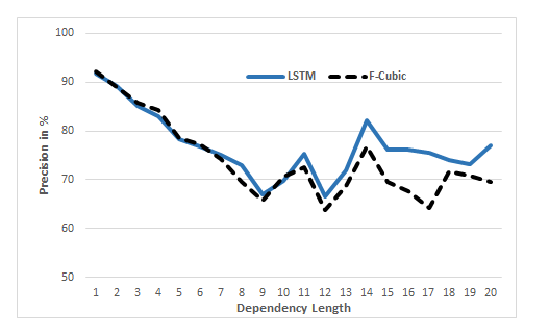
\includegraphics[width=.9\columnwidth]{images/precision.eps}
  \caption{Precision by Dependency Length}
  \label{fig:precision}
\end{minipage}
\begin{minipage}{.95\columnwidth}
  \centering
  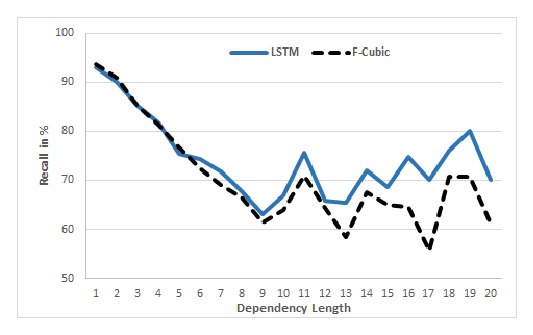
\includegraphics[width=.9\columnwidth]{images/recall.eps}
  \caption{Recall by Dependency Length}
  \label{fig:recall}
\end{minipage}
\end{figure*}
The LAS result on the Google Web Treebank is summarised on Table \ref{full_result_table}, where F-T and F-C represent the feedforward baselines with Tanh and Cubic activations, respectively.
Our LSTM model outperforms the feedforward baseline with the same Tanh activation function (87.5 vs 86.4 on WSJ Test), while achieving competitive accuracy with the Cubic baseline. 

We furthermore investigate the models' performance on long-range dependencies, reporting the result in terms of labelled precision and recall breakdown by dependency lengths on the WSJ test set in Table \ref{tab_long_range}. This result is also plotted in Figures \ref{fig:precision} and \ref{fig:recall}. 
Despite the models' similar overall accuracy, our LSTM model outperforms the Cubic baseline by more than 3\% in both precision and recall for dependency lengths greater than 7, and that the LSTM's performance degrades more slowly as dependency length increases.
%\footnote{Long-range dependencies only comprise 10\% of overall arcs, leading to similar overall accuracy}. 

%Since we did not tune on the web domains' dev set, we only show the test results of the web domains, using the "eval.pl" script for all final evaluation.

\begin{table}[t]
\centering
\begin{tabular}{|c|c|c|c|}
\hline
{\bf WSJ} & {\bf F - T} & {\bf F - C} & {\bf LSTM} \\ \hline
Dev             & 86.0        & 87.2        & {\bf 87.8} \\ \hline
Test            & 86.4        & {\bf 87.5}  & {\bf 87.5} \\ \hline \hline
{\bf Web Test}       & {\bf F - T} & {\bf F - C} & {\bf LSTM} \\ \hline
Answers         & 74.1        & {\bf 74.9}  & 74.6       \\ \hline
Emails          & 74.6        & {\bf 75.6}  & 74.4       \\ \hline
Newsgroups      & 79.3        & 79.9        & {\bf 80.2} \\ \hline
Reviews         & 76.5        & {\bf 77.2}  & 77.0       \\ \hline
Weblogs         & 80.7        & 81.1        & {\bf 81.2} \\ \hline
%{\bf Web Avg}   & 77.0        & {\bf 77.7}  & 77.5       \\ \hline
\end{tabular}
\caption{Google Web Treebank LAS Result}
\label{full_result_table}
\end{table}


%We additionally investigate the model's performance in identifying long-range dependencies. Such dependencies have proved difficult for most greedy transition-based parsers (McDonald and Nivre, 2007), including our feedforward baselines, that train on each oracle independently. This difficulty can be attributed to two main reasons: 1) most long-range dependencies are ambiguous, while the classifiers only have access to a limited context window, and 2) longer arcs are constructed after shorter arcs in transition-based parsing, thus increasing the chance of error propagation. In contrast, our LSTM model has two key advantages of modelling \textit{whole sequences} of training oracles, along with the theoretical ability to memorise all past context information, both of which are beneficial for longer dependencies.

\begin{table}[t]
\centering
\begin{tabular}{|c|c|c|c|c|}
\hline
{\bf \begin{tabular}[c]{@{}c@{}}Dep.\\ Length\end{tabular}} & \multicolumn{1}{l|}{} & F - T & F - C      & LSTM       \\ \hline
\multirow{2}{*}{1}                                          & Precision             & 91.4  & {\bf 92.2} & 91.7       \\ \cline{2-5} 
                                                            & Recall                & 93.1  & {\bf 93.6} & 93.0       \\ \hline
\multirow{2}{*}{2}                                          & Precision             & 87.9  & 88.9       & {\bf 89.3} \\ \cline{2-5} 
                                                            & Recall                & 90.3  & {\bf 91.0} & 90.1       \\ \hline
\multirow{2}{*}{3-6}                                        & Precision             & 81.7  & {\bf 83.4} & 82.6       \\ \cline{2-5} 
                                                            & Recall                & 79.2  & 81.3       & {\bf 81.4} \\ \hline
\multirow{2}{*}{7-49}                                       & Precision             & 68.1  & 70.3       & {\bf 73.5} \\ \cline{2-5} 
                                                            & Recall                & 62.6  & 65.6       & {\bf 69.5} \\ \hline
\end{tabular}
\caption{Long-range Arcs Precision \& Recall}
\label{tab_long_range}
\end{table}




\subsection{Regularisation Experiments}\label{hyperparameters}

We discover that regularisation is important for the LSTM parser, more so than feedforward architectures. Table \ref{table:with_without_dropout} compares the relative improvement due to dropout for feedforward vs. LSTM by constraining both models to have the same number of 500,000 parameters, corresponding to 50 hidden units for LSTM.
Observe that LSTM becomes competitive only with dropout. 

%Lastly, we investigated the impact of dropout on the performance of both the LSTM model and the Cubic baseline on the WSJ Test UAS. For the models without dropout, we trained the Cubic baseline with all the same hyper-parameters, while we reduced the number of hidden units of the non-dropout LSTM to 50 so that both models had a similar number of 500,000 parameters \footnote{Without dropout, larger LSTM models overfit and performed worse, constraining the size of our network}. The result is presented in Figure \ref{fig:with_without_dropout}. 

\begin{table}[h]
\centering
\begin{tabular}{|c|c|c|c|}
\hline
{\bf } & no dropout & with dropout & {\bf $\Delta$} \\ \hline
F-Cubic    & 89.1        & 89.5        & {\bf 0.4} \\ \hline
LSTM       & 87.4        & 89.5  & {\bf 2.1} \\ \hline
\end{tabular}
\caption{\label{table:with_without_dropout} Effect of Dropout on UAS Accuracy}
\end{table}


%\begin{figure}[h]
%\centering
%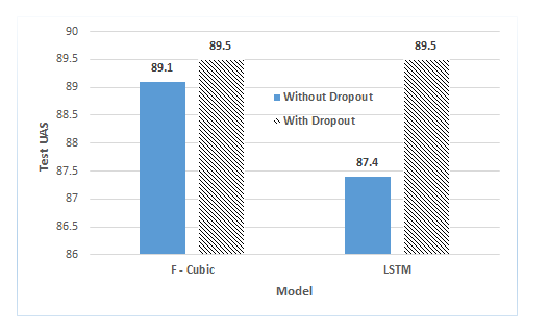
\includegraphics[scale=.95]{images/With_without_dropout.eps}
%\caption{Effect of Dropout on Accuracy}
%\label{fig:with_without_dropout}
%\end{figure}
%Despite the models' similar number of parameters, dropout significantly increased the LSTM model's accuracy, but not on Cubic baseline's. This result suggests that the LSTM model crucially requires regularisation to generalise well, which we investigate further in subsection \ref{hyperparameters}.

%Based on the previous finding, we empirically investigate various regularisation settings for the LSTM model and the correlation with hidden layer size. %We leave the analysis of other variations, such as optimisation method and LSTM architectures (e.g. peephole connections), to future work.

%To investigate what kind of dropout is beneficial,  we conducted further experiments on a subset of the training data (the first 80,000 tokens of the WSJ training set). We used the same experimental settings as in Subsection \ref{exp_settings_large} and evaluate UAS on the full WSJ dev and test set.
%except that training was done for a maximum of 500 epochs and stopped early if no better dev accuracy was found after 50 consecutive epochs. 
%\footnote{the UAS is calculated using the parser's internal evaluation, which might differ with the eval.pl script result}

To investigate what kind of dropout is beneficial,  we conducted further experiments on a subset of the training data (the first 80,000 tokens of the WSJ training set).\footnote{We used the same experimental settings as in Subsection \ref{exp_settings_large} and evaluate UAS on the full WSJ dev and test set, with hidden layer size fixed at 60.}
The results of dropout and L-2 regularisation are in Table \ref{tab_regul}, along with the epoch where the best dev UAS is found. E-H and H-O indicate dropout between the embedding-hidden and hidden-output connections, respectively. %For L-2, we performed a grid search in the log-linear space for L-2 coefficients between $10^{-3}$ and $10^{-8}$. For dropout, we experimented with three dropout rates: 0.2, 0.4, and 0.6, and apply each rate on three alternatives: on the embedding-hidden (E-H) connections, on the hidden-output (H-O) connections, and on both the embedding-hidden and hidden-output (E-H + H-O) connections. .

\begin{table}[t]
\centering
%\captionsetup{justification=centering}
\begin{tabular}{|c|c|c|c|c|}
\hline
\multicolumn{2}{|c|}{{\bf Reg Settings}} & {\bf Dev } & {\bf Test } & {\bf Epoch} \\ \hline \hline
\multicolumn{2}{|c|}{{\bf L2 $\lambda$}}    &               &                &             \\ \hline
\multicolumn{2}{|c|}{0}                  & 80.2         & 80.0           & 42          \\ \hline
\multicolumn{2}{|c|}{$10^{-8}$}                  & 80.7          & 80.8          & 25          \\ \hline
\multicolumn{2}{|c|}{$10^{-7}$}                  & 79.9          & 80.3           & 43          \\ \hline
\multicolumn{2}{|c|}{$10^{-6}$}                  & 79.8          & 80.1           & 43         \\ \hline
\multicolumn{2}{|c|}{$10^{-5}$}                  & 80.5          & 80.4          & 46          \\ \hline
\multicolumn{2}{|c|}{$10^{-4}$}                  & {\underline{83.4}}          & {\underline{82.9}}           & 206          \\ \hline
\multicolumn{2}{|c|}{$10^{-3}$}                  & 81.6          & 81.6           & 159          \\ \hline \hline
\multicolumn{2}{|c|}{\bf Dropout $p_{drop}$}  &               &                &             \\ \hline
\multirow{3}{*}{E-H}      & 0.2          & 84.4          & 84.3          & 97          \\ \cline{2-5} 
                          & 0.4          & 85.8          & {\underline{85.7}}           & 257          \\ \cline{2-5} 
                          & 0.6          & {\underline{\bf 86.2}}         & 85.5           & 273          \\ \hline
\multirow{3}{*}{H-O}      & 0.2          & 81.8          & 81.6          & 52          \\ \cline{2-5} 
                          & 0.4          & {\underline{82.3}}          & {\underline{82.1}}          & 93          \\ \cline{2-5} 
                          & 0.6          & 81.9          & 81.7          & 69          \\ \hline
\multirow{3}{*}{Both}  & 0.2          & 85.4          & 85.0          & 122          \\ \cline{2-5} 
                          & 0.4          & {\underline{86.1}}         & {\underline{\bf 85.9}}           & 315          \\ \cline{2-5} 
                          & 0.6          & 85.3          & 85.3           & 500          \\ \hline
\end{tabular}
\caption{UAS Accuracy of Various Regularisation}
\label{tab_regul}
\end{table}

While dropout generally results in slower convergence, the technique outperforms L-2 and significantly improves the model's accuracy by more than 6\%. Most importantly, we found input dropout to be more crucial than hidden-output dropout and achieves the same accuracy as dropout on both input and hidden layers, suggesting that our model can achieve good accuracy with input dropout alone. %\footnote{In contrast, hidden layer dropout is much more important for the feedforward model, and high input dropout rates hurt the feedforward model's performance}. 
We found dropout rates between 0.4 and 0.6 to be effective.
Further, we found that dropout generally improves LSTMs regardless of model size. Figure \ref{fig:dropout_hidden} shows how dropout of 0.5 on E-H and E-O layers improve results for various hidden layer sizes. 

\begin{figure}[t]
\centering
  \centering
  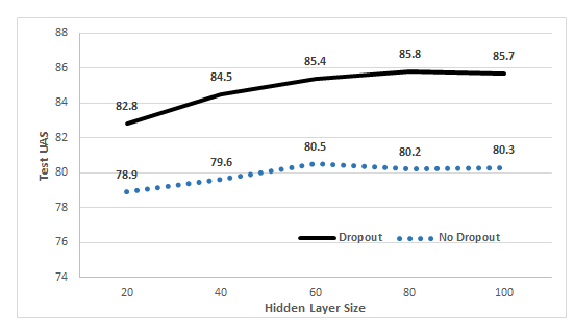
\includegraphics[width=.9\columnwidth]{images/dropout_hidden.eps}
  \caption{UAS Accuracy vs Hidden Layer Size}
\label{fig:dropout_hidden}
\end{figure}
%To investigate the correlation between dropout and hidden layer size, we applied a fixed dropout rate of 0.5 on both the embedding-hidden and hidden-output connections and experimented with hidden layer sizes from 20 to 100, in increments of 20. We compared the result with the models without dropout and summarised the test UAS result on Figure \ref{fig:dropout_hidden}. Importantly, dropout resulted in a sizable improvement even for small hidden layer sizes that are less prone to overfitting. This result indicates that dropout greatly improves generalisation ability and should be used regardless of model size. 
